\begin{frame}{The BNP Model \citep{sethuraman:1994:constructivedp}}
A {\bf Dirichlet process prior} allows for an infinite number of components.
\vspace{-0.2em}
\begin{figure}[!h]
\centering
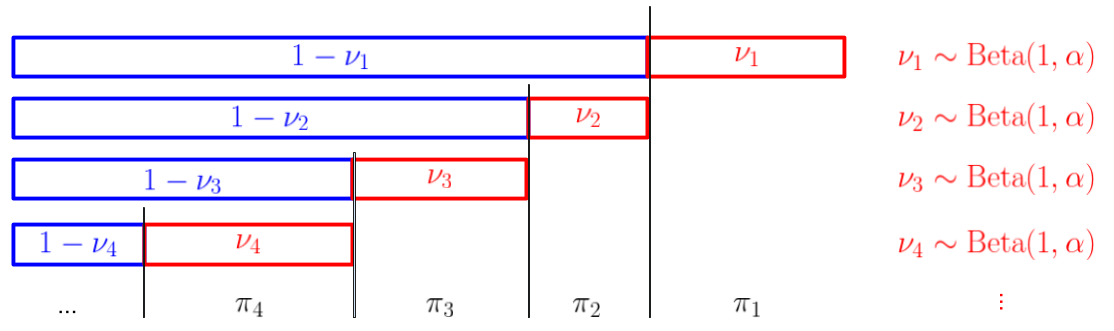
\includegraphics[width = 0.95\textwidth]{./static_figures/DP_stick_breaking.png}
\caption{A schematic of the Dirichlet process prior}
\end{figure}
\vspace{-0.2in}

While there are an infinite number of {\bf components}, there are a finite number of {\bf clusters} in a given dataset. 
%\pause 

Posterior quantities depend on the BNP prior, which is defined 
by the density of the stick-breaking process $\nuk \sim \p(\nuk)$.


% \begin{enumerate}[(1)]
% \item How many clusters are in the {\itshape current} dataset?

% %\pause
% \item How many clusters would we expect to see in a {\itshape new} dataset?
% \item Which observations in the current dataset cluster together?

% \end{enumerate}

% \pause

% These quantities depend on the choice of stick-breaking prior.

%\pause

\vspace{1em}

\begin{mdframed}[style=MyFrame]
\begin{center}
{\bf If $\nuk \sim \betadist{1, \alpha}$ what should $\alpha$ be?\\}
{\bf Why should $\p(\nuk)$ even be in the Beta family?}
\end{center}
\end{mdframed}

\end{frame}
